\documentclass{minimal}
\usepackage{tikz}

\begin{document}
	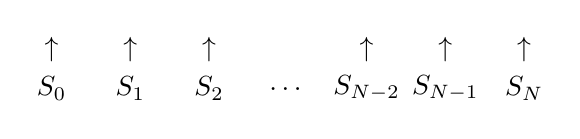
\begin{tikzpicture}{
		\def\verticalspacing{0.5}
		\def\N{6}

		\foreach \i in {0,...,2}
		{
				\pgfmathparse{rnd >= 0.5 ? 3 : 5}\pgfmathresult
				
				\node (S_\i) 		at (\i,0) {$S_\i$};
				\node (S_\i arrow) 	at (\i,\verticalspacing) {$\uparrow$};
		}
		\pgfmathtruncatemacro{\position}{(\verticalspacing) / 2}
		\node (ellipsis) at (3,\position) {\dots};
		\foreach \i in {2,...,1}
		{
				\pgfmathtruncatemacro{\position}{(\N - \i}
				\node (S_Nmin\i) 		at (\position,0) {$S_{N - \i}$};
				\node (S_\i Nminarrow) 		at (\position,\verticalspacing) {$\uparrow$};
		}
		\node (S_Nmin6) 			at (\N,0) {$S_{N}$};
		\node (S_6Nminarrow) 		at (\N,\verticalspacing) {$\uparrow$};

	}\end{tikzpicture}
\end{document} 